\section{Methodology}
Link iO to boolean circuit and tell what we are trying to achieve.

\subsection{Hypothesis}
Thomborson proposed a space-efficient and computationally-appropriate file format (BPW) for the evaluation of very large Boolean functions with bounded program width\cite{clark}. Gates of a circuit are represented by descriptors holding information about their type (AND, OR, $\dots$) and are sequentially encoded inside the file's body. In our experiment we generate random boolean circuits (evaluating a random boolean function) with various width $w = \{ 10^3, 10^4, 10^5, 10^6, 10^7, 10^8\}$ for a fixed circuit size $N = 10^8$. The widest circuit has depth 1. The generated circuits are represented using a simplified BPW format by storing the gate type and the input indices only and by making some assumptions about the properties of circuit under test. In particular, we make the following assumptions about the size of the circuit's inputs and outputs as well as the manner outputs from level $L_i$ are passed to gates of level $L_{i+1}$ as inputs.
\begin{enumerate}  
\item All circuits have size $N = 10^8$
\item A circuit input array has size $w$.
\item Any given level $L$ has exactly $w$ gates.
\item Every gate has only one output.
\item A circuit output array has size $w$.
\item Any given gate from a level $L_i$ has between one and three inputs that come from level $L_{i-1}$ exclusively. We can write the following:\break $G_i = f(X)$ where $f$ is a boolean operator and $X$ is an 8-byte array of size 1, 2 or 3. 
\item The output of a gate is written inside the output array at the same index of the gate. $G_i(X) = Output$ $array[i]$.
\end{enumerate}
A circuit evaluation is sequential at both gate and layer level. A Level $L_i$ is presented with an input array of size $w$ that corresponds to the output array of level $L_{i-1}$. Gates of $L_i$ are processed in ascending order of index in the level. Every gates retrieves its relevant inputs as described by the gate descriptor. Inputs indices for a gate are randomly distributed over $[0, w-1]$. We believe that this randomness will severely affect the overall performance of the circuit for large $w$ where the entire input array cannot fit in the cache. Once a gate is processed, its output is stored in the output array at the same index as the gate. Once all the gates of level $L_i$ are processed, the execution cursor moves to level $L_{i+1}$.
\par
\begin{figure}[h]
	\center
	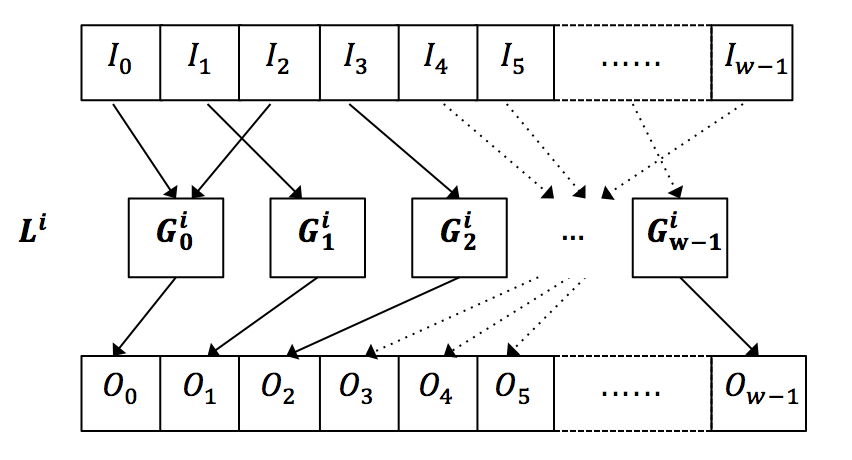
\includegraphics[width=0.8\textwidth]{img/level.png}
	\caption{Simple description of Level $L_i$ evaluation}
\end{figure}
\par
We predict that the total running time of a circuit follows this analytical model:
\begin{equation}
T = \max\{ t_g + t_e, t_m(w) \}
\end{equation}
where $T$ is the total elapsed (wallclock) time per gate, $t_g$ is the CPU time for generating a gate, $t_e$ is the CPU time for evaluating a gate, and $t_m(w)$ are the memory-stalls from the gate-generation and gate-evaluation computations.
\par
In our experiment, we generate the entire circuit prior to its evaluation. $t_g$ is in fact related to the time cost of loading of the gate for execution. We assume that this time component is near constant per gate and is not affected by the width $w$. The generation step executed initially is not monitored for performance. The resulting circuit is stacked gate by gate in a simplified BPW file. Following the initial BPW model the first 4 bytes represent the header of the a BPW file\cite{clark}. The following bytes represent the total gates of the circuit. All gates are sequentially represented from index $0$ to index $10^8-1$. A given gate's encoding varies from 9 to 25 bytes. The first byte holds the type of the gate. The following 8 to 24 bytes present the input indices encoded over 64-bits each. We could optimise the gate's representation further to compress a gate's representation but we kept this current model for simplicity. Since we fixed the size of the circuits under test to $N = 10^8$, the average size of a circuit stored in a BPW file is $avg(sizeof(Gate)) * 10^8 \approx 2 GB$ \footnote{We modelled 14 types of Gates; 1 $\times$ 1-input, 6 $\times$ 2-input and 7 $\times$ 3-input gates. On average, a gate has 2.43 inputs encoded with 8 bytes per input plus one byte for the gate type.}.
\par
We used the \textit{perf} linux command to measure the impact of evaluating a circuit on the CPU. \textit{perf} is a tool written in C that uses Performance Counters to profile an application. Performance counters are CPU hardware registers that count hardware events such as instructions executed, cache-misses suffered, or branches mispredicted\cite{perf}. In particular, the \textit{perf stat} subcommand allows to obtain event counts that are of interest to our experiment. These events are mainly \textit{instructions, cycles, LLC-loads} and \textit{LLC-misses}. For every value of $w$, we configure \textit{perf} to run the experiment 3 times and collect the average counts.


\par
TODO
\par
If Tw is too small (define too small) then Tw is negligible comparing to Ta and Tb. However, starting from a particular threshold, Ta + Tb become negligible relatively to Tw.
Equation x summarises our analysis of the performance of our benchmark:
\par
Eq here

From the results collected, we can observe that when $w < 10^7$, $t_m(w) < t_g + t_e = 130$ ns and when $w >= 10^7$, the computation becomes memory-bound, allowing us to estimate $t_m(10^7) = 162$ nsec and $t_m(10^8) = 176$ nsec.

\subsection{Generation  And Execution Time}
The $t_g + t_e = 130$ nsec estimate seems reasonable: it is about 45 CPU clocks. Assuming no stalls, a dual-issue CPU clocked at xxGHz can execute up to 90 instructions during that time. Our testing plateform has an x86 instruction and the observed issue rate is relatively stable at 1.7 inst/clock for all tested $w < 10^7$.  This is not a surprisingly-low (nor a surprisingly-high) issue-rate for a dual-issue i586.  We could also estimate the instructions per gate at  1.7*45 = 75 instructions.
\subsection{Memory Time}
Regarding $t_m(w)$: about half of your gates are 3-input and half are 2-input, so there'll be about 2.5 memory-fetches per gate-eval (to read its inputs).  There'll also be some memory-writes during the gate-evaluation process (when you're unpacking the gate-descriptors), some memory-reads (when you're reading the unpacked gate-descriptions); and you'll be writing the gate-output bits.   You *might*

Your gates are unpacked into a top-level struct of 16 bytes (after padding to the next-larger power of two), and each gate references 1 to 3  input-descriptors of 8 bytes each (these are packed in the "inputs" array).  At 2.5 inputs/gate that's 20 bytes for the input-descriptors plus 16 bytes for the top-level gate-descriptor -- a total of 36 Bytes per gate, or 36e8 = 3.6 Gbytes per level when $w=10^8$.  It's certainly not cache-resident and if you had only 4 GB of main memory there'd be some "hard" page-faults requiring disk activity.  But you're probably (just) ok here; once again it'd be a good idea to avoid unpacking a gate-descriptor from a BPW file until you're ready to evaluate it, rather than unpacking an entire level...

The gate input-reads are scattered more or less randomly through an array of $w$ bits -- so they're almost-always an LLC miss for any $w$ large enough that this bit-array doesn't fit in your 6MB = 48 Mb LLC, i.e. whenever $w > 10^7$.   The miss rate should be very close to (48e6/1e8) = 48\% for w=1e8.   With 1 gate eval every 176 nsec, and (2.5)(48\%) = 1.2 misses/gate-eval, that's a memory-latency of 176/1.2 = 147 nsec per LLC miss.   That's in range of the (indicative) latency data I see in point 4 of https://software.intel.com/en-us/articles/intelr-memory-latency-checker -- and your memory is pretty heavily loaded for bandwidth, from these gate-input reads and also from the gate-descriptors.

So... the model seems plausible... however we'd have a significantly-lower miss rate if your gate input-reads aren't actually scattered randomly through an array of $w$ bits, due to a defect in your random-number generation.

As for the possibility that your reads and writes of unpacked gate-descriptors are causing a memory-bandwidth bottleneck... each level of a $w=10^8$ circuit takes 36e8 bytes to store its gates in unpacked format.  That's a total of 2*36e8B/17.6s = 410 MB/s in memory bandwidth.  Your performance monitor reports "28.817 M/sec" for the LLC-load rate.  I have *no idea* whether these are 32B loads or 16B loads or 64B loads -- but if they're 32B loads then we get 922 MB/s.  That leaves 510 MB/s for the gate-input reads, at 32B per LLC miss.  Above I estimated one LLC miss on the gate-input reads every 147 nsec: that's 217 MB/s.  Dunno what's happening for the other 300 MB/s, but there will be some additional traffic, so it's an ok explanation even though it'd be good to have some story to tell about this 300 MB/s of "other" memory bandwidth...

If each LLC load is 16B, then your perf-counts are reporting 461 MB/s of memory bandwidth, leaving only 51 MB/s for the gate-input reads.  At 16B per LLC miss, these add up to about 108 MB/s -- so if an LLC load is 16B the data is not well-explained by the analysis above.

I have to go now... I hope this made some sense!  The idea is for you to tell some story, along the above lines, about your observations.  If you're unable to explain some aspects of your data, that's fine, you're certainly not expected to be an expert in performance-modelling of memory systems!  Instead you should "keep it simple" in your explanations and raise some questions (in your analysis) which merit further study.